\chapter{Paper III:\@
  Overreact, an in silico lab:
  \linebreak automative quantum chemical microkinetic simulations
  for complex chemical reactions
 }%
\label{ch:paper3}

\fullcite{Schneider2022}

% Abstract
Present work introduces a novel Python package overreact to propagate chemical reactions over time using computational chemistry data.
A novel Python package is presented to predict time-dependent chemical reactions from computational chemistry data.

% Introduction
Developing catalysts and machines to meet the challenges of the 21st century through improved understanding of reaction mechanisms.
Accurate and efficient computational modelling tools and methodologies have enabled the calculation of complex reaction mechanisms and elucidation of experiments, aiding the comprehension of complex chemical phenomena.
Complex physical effects must be considered to computationally model chemical reactions.
Rate constants influence outcome and selectivity of competing reactions, but also concentrations and types of steps can affect rate laws.
Simulating reactions via microkinetic simulations to take concentration effects into account, and first-principle calculations for binding free-energies and reaction rate constants provide insight on complex reaction phenomena.
No general solution exists to generate a reaction rate ODE system with quantum tunneling approximations from an arbitrary scheme.
% Table comparing programs
The table demonstrates relationships between different programs for theoretical chemical kinetics, such as the language the program is coded in and the theories it can be applied to. For example, MultiWell and Pilgrims are both coded in Fortran and can be applied to the TST, VTST and RRKM theories, while APUAMA is coded in C++ and supports only TST theory. The programs also differ in their molecularity, phases and supported tunnel effects, such as Wigner, Eckart, etc. For example, Polyrate can be applied to the TST and VTST theories with uni/bi-molecularity and on gas, solid and gas-solid phases, while MESMER works with only uni-molecularity and gas and solution phases.
%
A robust software, \overreact, is introduced to solve chemical reaction networks automatically with outputs from quantum calculations.
\overreact is a user-friendly Python program and library that generates and solves chemical kinetic ODEs, allowing the user to adjust first-principle absolute Gibbs energy errors.

% Methodology
Automatically builds chemical microkinetic models from first principle calculations.
Equations and initial concentrations yield concentrations of all species over time.
Dataflow diagram is simplified overview of library's features in Supporting Information.

% Results and discussion
Results of \overreact usage with default settings are presented in subsections.
% - Simple gas-phase autoisomerizations
Reaction rates of simple autoisomerization reactions are estimated precisely using \overreact.
Estimated autoisomerization rate of ethane from staggered to eclipsed and back to staggered was found to agree with experimental value.
The reaction rate constant for the umbrella inversion of ammonia was estimated to agree with experimental values of $4 \times 10^{10}$~s$^{-1}$.
Tanaka \cite{Tanaka_1996} studied methane degradation by chlorine radicals in the atmosphere; the reaction rate constant was consistent with the experimental value of $1.0 \times 10^{-13}$~cm$^3$~molecule$^{-1}$~s$^{-1}$~\cite{Burkholder_2020}.
% - Examples in solution
Algorithm creates fictitious reaction rate constants that guarantee equilibrium is satisfied, allowing simultaneous study of both fast reactions and equilibria.
Equilibria can provide qualitative insight and be used to obtain Boltzmann populations with constraint optimization.
We estimated acetic acid-acetate concentrations using a combination of \emph{ab initio} calculations, experimental pK$_a$ values and \ce{H+} concentration constraining.
Optimizations and frequencies for \ce{AcOH(aq)} system performed concluding with predictions of reaction concentrations of both solvation energies.
\overreact produces the expected result if given precise energy values.
M06-2X-D3(0)/6-311++G(d,p)/SMD was used to calculate a rate constant for \ce{NH3_{(w)} + OH._{(w)} -> NH2._{(w)} + H2O_{(w)}}.
Experiments were done at high pH and unaffected by ammonia-ammonium equilibrium for simplicity.
\citeauthor{P_rez_Soto_2020} applied computer-aided analysis to elucidate an imine formation reaction, taking into consideration water contamination from residuals in the solvent or from a by-product.
Reactions can be complex and require microkinetics or other techniques to properly explain them.
\citeauthor{P_rez_Soto_2020} investigate systematic errors in bimolecular reaction barriers and suggest a method for reducing them using a single tunable parameter.
Experimental data compared to Perez-Soto's work in \cref{fig:perez-soto-bias=3.2} (ADD FIGURE).
Used energy correction of 3.2~kcal~mol$^{-1}$ for RMSE of 4.97~mM; additional approximations (Eckart, quasi-rigid rotor-harmonic) applied.
Progress is being made to fit systematic deviations in first-principles reaction schemes by using available experimental data.
Intramolecular amide hydrolysis mechanisms is investigated with calculations and experimentally derived pK$_a$ of acetic acid, with 3 proposed mechanisms replicated.
Proton transfer in a four-membered ring transition state through \ce{I^$\ddagger$} is rate-determining, facilitated by proton shuttle and active participation of the solvent.
Reaction occurs in acidic environments only, studied at different pH values.
The system simulates 25 simultaneous reactions and 17 species, with results matching those of related systems at pH 5.
Simulations show conversion under these conditions happens mostly via equilibrium-state \ce{C}, rest-state \ce{J} and the help of solvent elongating the \ce{C-N} bond.

% Conclusions
Automatically obtaining reaction kinetic profiles from first principles and adjusting any disparities through energetic biases to improve accuracy with bimolecular systems.
Overreact provides a complete and simple predictive environment for chemical kinetics and catalysis that enables the inference of reaction rate constants from microkinetic simulations.
This article presents an open-source package to explore and analyse reaction mechanisms. Future developments aim to predict catalysts performance at a larger scale.

MY TEXT GOES BELOW.

\overreact is a software package for microkinetic modelling using data from
first-principles quantum chemical
calculations~\cite{Schneider2022,overreact2021zenodo}.
It is an improvement on a first attempt to build a
chemical chemical kinetics simulator that uses first-principles quantum
chemical calculations~\cite{pyrrole2019zenodo} (for a list of other software
contributions that have taken place during the course of the PhD, see~\cref{ch:all-works}).
Lessons learned from this first iteration, as well as the methodology
underlying \overreact, can be found in~\cref{sec:overreact-methods}.

The methology was developed such that as much as possible of the physics of the problem could be included,
while still making the whole process manageable from the computational point of view.
This means choosing the use of classical transition state theory,
whose requirement of having transition state structures is attainable
using simply available computational chemistry packages of today, in contrast to other theories
such as variational transition state theory.
Although limiting, this way of doing things is accurate to a wide variety of chemical phenomena.
% TODO: CITATION FOR THE PHRASE ABOVE!

The literature is well-stablished in most of this regard.
For instance, CITE SUCH AND SUCH, theories of transition state, etc.
RRKM, Marcus theory, VTST, etc.
On other aspects, such as solvation entropy, it is actually divided CITE.\@

Regarding the emergent need for mechanistic elucidation, the research shows promissing
results in terms of doing semiautomatic hypothesis test in terms of which reactions are feasible
in a given context.
As far as we known, this is the first system that is able to produce kinetic reaction profiles
automatically from simple computational chemistry outputs and still take into account most of the physics of the problem.

% TODO: get that from the paper! There's a table for it!
But many contributions came earlier, for instance SUCH AS SUCH.\@
Polyrate, EyringPy, MKMCXX, etc.
CITE Emílio Martínez?

It is important to do this investigation, as the demand has considerably increased throughout the years.
One can not expect to produce excellent catalytic processes without knowning how they work,
especially if there is need to \emph{systematically} and \emph{consistently} design them for various applications.
This is extremelly important in today's economy and ongoing climate crisis.

Relatedly, health applications are of utmost importance, as the world's population gets steadily older.
In this respect, cancer therapies are very important as well.

Allowing rapid rational design and investigation in those areas where understanding how reactions work is important
is a crucial effort of this work.

We aimed towards making it extremelly easy for computational discoveries in the elucidation of reaction mechanisms
to be compared with experimental data.
In this scope, one restrained the set of approachable systems to ones
being specifically investigable with today's availability of computational chemistry packages.
Although reasonably general, the method does not cover surface reactions,
some condensed state effects such as solvation entropy,
pressure-dependent reactions,
very fast reactions,
diffusion-controlled reactions,
reactions that transit between potential energy surfaces such as photochemical ones, and more.
Fully covered are room-temperature reactions in gas and solvated phases in the infinite dilution approximation.

A variety of methods were employed.
We get energies from computational chemistry packages,
together with vibrational frequencies.
Together with the molecular structure,
one is able to calculate the molecular partition function for such systems.
This allows one to calculate Gibbs' free energies and, together with reaction hypotheses,
activation free energies for such reactions.
This, together with tunneling approximations, one is able to produce accurate reaction rate constants.
% TODO: things missing for above: symmetries, etc., Grimme's stuff, etc.

% TODO: useful for
One could inspect steady-state conditions, in which the concentrations and rates have converged to some final value,
search for the most predominant species under catalytic conditions, computationally estimate the overall turn-over frequency,
an essential measure of catalytic activity, and understand selectivity of a catalysts towards particular products.
Not only it provides insight into concentration dependencies and comparison with experiment,
such framework would serve as a benchmark for hypothesis testing, allowing the prediction of chemical behaviour in a computationally affordable and precise way.
Kinetic models in such a framework can be progressively constructed, with a single pathway added at a time until a match with the experiment,
simplifying the workflow, easing the computational burden and increasing efficiency, as was recommended elsewhere~\cite{Jara_z_2019}.
Such an incremental modeling protocol is arguably maximally efficient, as a
minimal set of reactions lead to more easily rationalisable and
``probably less wrong'' models~\cite{Blackmond_2015,Jara_z_2019}.

\section{Paper}

The publication can be read in full next.
Reprinted with permission from
\fullcite{Schneider2022}.
Copyright
\citeyear{Schneider2022}
John~Wiley~\&~Sons,~Inc.

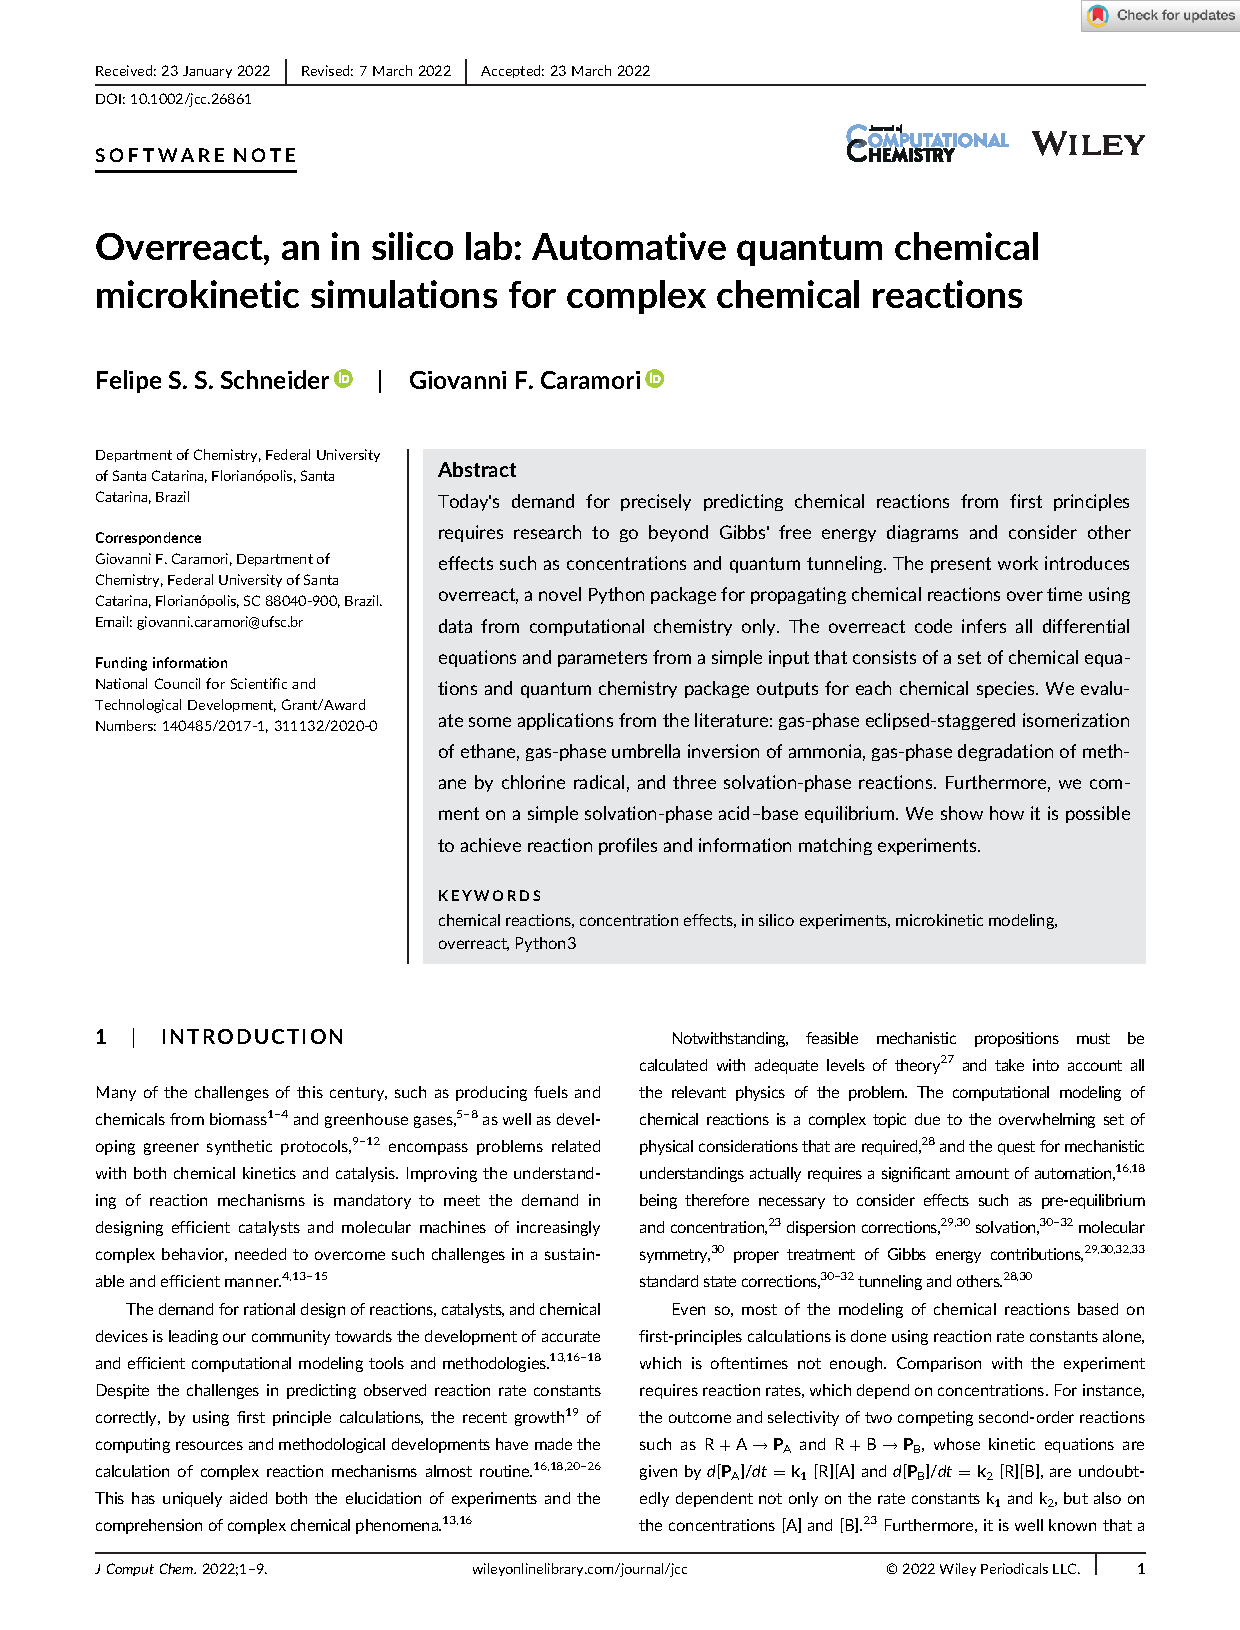
\includepdf[pages=-]{pubs/schneider2022-paper3.pdf}
